\chapter{Performance of Our Driver}
\label{chap:performance}
\todo{todo}

To compare the performance of our driver to BitLocker and VeraCrypt, we conducted several experiments measuring the throughput for sequential and random-access reading. The tests were done both in a virtual machine and on real hardware.

\section{Experimental Setup and Design}
\label{chap:performance.setup}
Both the setup for the virtual machine and the real hardware will be described in this section. They are mostly the same, so when not stated otherwise, the contents in this section apply to both.

For each encryption technique featured in our benchmarks we created a separate 5 GiB FAT32 volume on the same \todo{disk/SSD}, as shown in \autoref{fig:performance.setup.disklayout}. Every volume contained the same file, \texttt{random.bin} (4 GiB of random data). \todo{if HDD: 1 GiB}

\begin{figure}[htb!]
	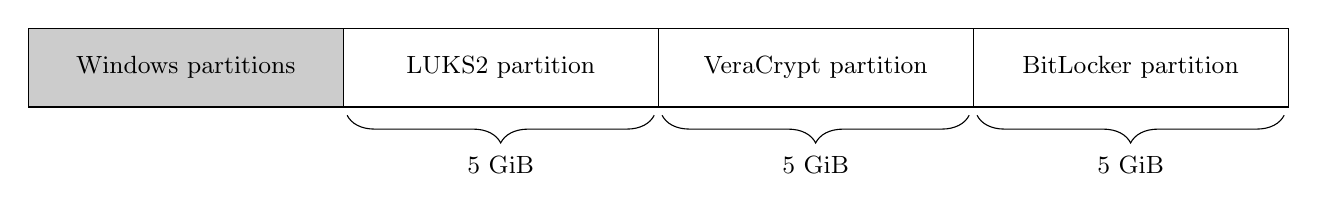
\begin{tikzpicture}
		\draw [fill={gray!40}] (0, 0) rectangle (4, 1);
		\node [anchor=center] at (2, 0.5) {\small\makecell{Windows partitions}};
		\draw [fill=white] (4, 0) rectangle (8, 1);
		\node [anchor=center] at (6, 0.5) {\small\makecell{LUKS2 partition}};
		\draw [fill=white] (8, 0) rectangle (12, 1);
		\node [anchor=center] at (10, 0.5) {\small\makecell{VeraCrypt partition}};
		\draw [fill=white] (12, 0) rectangle (16, 1);
		\node [anchor=center] at (14, 0.5) {\small\makecell{BitLocker partition}};

		\draw [decorate, decoration={brace, amplitude=10pt, mirror}, yshift=-3pt]
		(4.05, 0) -- (7.95, 0) node [black, midway, yshift=-18pt] {\small 5 GiB};
		\draw [decorate, decoration={brace, amplitude=10pt, mirror}, yshift=-3pt]
		(8.05, 0) -- (11.95, 0) node [black, midway, yshift=-18pt] {\small 5 GiB};
		\draw [decorate, decoration={brace, amplitude=10pt, mirror}, yshift=-3pt]
		(12.05, 0) -- (15.95, 0) node [black, midway, yshift=-18pt] {\small 5 GiB};
	\end{tikzpicture}
	\caption[
		SSD partition layout
	]{
		SSD partition layout. This is the layout of the real hardware SSD. The layout of the \todo{HDD} was similar, but with additional Windows partitions behind the the encrypted volumes. The virtual machine had a virtual disk for the Windows installation and another one for the three encrypted volumes.
	}
	\label{fig:performance.setup.disklayout}
\end{figure}

To test the performance of the different drivers, we used the \texttt{fio} command line tool\footnote{\label{fn:performance.setup.fio} \url{https://fio.readthedocs.io}} to read from the three copies of \texttt{random.bin}, using different access patterns. Each run of \texttt{fio} is called a \emph{job}, and the configuration for a job is stored in a \emph{job file}.

\todo{fio options, job files, and powershell script}

\todo{(except for VM) every run three times and average it, if multiple threads the value used for one run was the average of all threads}

\todo{VM: fresh Windows 10 build 19043.928 install, virtualized using Oracle VirtualBox 6.1.22, 8 GiB of virtual RAM (backed by 16 GiB DDR4 RAM), 4 virtual cores (backed by a Intel Core i7-7700K), virtual SSD stored on a 250 GB Samsung SSD 850 EVO}

\todo{Real hardware: fresh Windows 10 build 19043.928 install, 8 GiB DDR3 RAM, Intel Core i7-3770 quad core with SMT, 233GiB SanDisk SDSSDH3250G}

\todo{keep \cite{Traeger2008} in mind}

\cite{Traeger2008}: ``[Random-access I/O] is typical of on-line transaction processing (OLTP) systems, database systems, or mail server applications.'' Examples for sequential access are ``large file processing (scientific computing, large-scale financial processing), large database queries (data mining, business intelligence), and on-demand video.''

\section{Virtual Machine Experiments}
\label{chap:performance.vmexperiments}
\todo{todo:} For testing purposes, we tried optimizing the performance by restricting support to AES256-XTS. This enabled removing some if-else constructs that dispatched de-/encryption functions based on whether AES128 or AES256 was used. Even though these conditionals were located in a performance critical section, we saw no speed improvements. Our theory for why this was the case is the following: our driver was only ever used for one LUKS2 partition and therefore always took the same path through the if-else (either always AES128 or always AES256). This trained the CPU's branch prediction on this one specific path. Thus, after a short training phase, the CPU always speculatively executed the correct path, resulting in the same performance as without the if-else.

\todo{todo:} The default compiler optimization settings in Visual Studio were a little bit conservative and also optimized for small code size rather than high speed/performance. After tuning these settings to enable more aggressive optimizations and also focus on speed rather than code size, we found that \todo{this is a little bit complicated...}.

\begin{figure}[htb!]
	\center
	\includegraphics[scale=1]{../fig/performance.vmexperiments.seq.pdf}
	\caption[
		Comparison of sequential read throughput in a virtual machine
	]{
		Comparison of sequential read throughput in a virtual machine. \todo{todo}
	}
	\label{fig:performance.vmexperiments.rand}
\end{figure}

\begin{figure}[htb!]
	\center
	\includegraphics[scale=1]{../fig/performance.vmexperiments.rand.pdf}
	\caption[
		Comparison of random-access read throughput in a virtual machine
	]{
		Comparison of random-access read throughput in a virtual machine. \todo{todo}
	}
	\label{fig:performance.vmexperiments.rand}
\end{figure}

\section{Real Hardware Experiments}
\label{chap:performance.hwexperiments}

\subsection{Unencrypted Throughput Measurements}
\label{chap:performance.hwexperiments.unencrypted}
\begin{figure}[htb!]
	\center
	\includegraphics[scale=1]{../fig/performance.hwexperiments.nullcryptoseq.pdf}
	\caption[
		Unencrypted versus null-crypto sequential read throughput
	]{
		Unencrypted versus null-crypto sequential read throughput. \todo{todo}
	}
	\label{fig:performance.hwexperiments.nullcryptoseq}
\end{figure}

\begin{figure}[htb!]
	\center
	\includegraphics[scale=1]{../fig/performance.hwexperiments.nullcryptorand.pdf}
	\caption[
		Unencrypted versus null-crypto random-access read throughput
	]{
		Unencrypted versus null-crypto random-access read throughput. \todo{todo}
	}
	\label{fig:performance.hwexperiments.nullcryptorand}
\end{figure}

\subsection{First Series of Encrypted Throughput Measurements}
\label{chap:performance.hwexperiments.encryptedseries1}
\begin{figure}[htb!]
	\center
	\includegraphics[scale=1]{../fig/performance.hwexperiments.beforeoptseq.pdf}
	\caption[
		Comparison of sequential read throughput
	]{
		Comparison of sequential read throughput. \todo{todo}
	}
	\label{fig:performance.hwexperiments.beforeoptseq}
\end{figure}

\begin{figure}[htb!]
	\center
	\includegraphics[scale=1]{../fig/performance.hwexperiments.beforeoptrand.pdf}
	\caption[
		Comparison of random-access read throughput
	]{
		Comparison of random-access read throughput. \todo{todo}
	}
	\label{fig:performance.hwexperiments.beforeoptrand}
\end{figure}

\subsection{Second Series of Encrypted Throughput Measurements}
\label{chap:performance.hwexperiments.encryptedseries2}
\todo{all the different optimizedv2 graphs}

\begin{figure}[htb!]
	\center
	\includegraphics[scale=1]{../fig/performance.hwexperiments.optseq.pdf}
	\caption[
		Comparison of sequential read throughput (optimized \texttt{luks2flt})
	]{
		Comparison of sequential read throughput (optimized \texttt{luks2flt}). \todo{todo}
	}
	\label{fig:performance.hwexperiments.optseq}
\end{figure}

\begin{figure}[htb!]
	\center
	\includegraphics[scale=1]{../fig/performance.hwexperiments.optrand.pdf}
	\caption[
		Comparison of random-access read throughput (optimized \texttt{luks2flt})
	]{
		Comparison of random-access read throughput (optimized \texttt{luks2flt}). \todo{todo}
	}
	\label{fig:performance.hwexperiments.optrand}
\end{figure}

\begin{figure}[htb!]
	\center
	\includegraphics[scale=1]{../fig/performance.hwexperiments.optseqqueue.pdf}
	\caption[
		Comparison of queued sequential read throughput (optimized \texttt{luks2flt})
	]{
		Comparison of queued sequential read throughput (optimized \texttt{luks2flt}). \todo{todo}
	}
	\label{fig:performance.hwexperiments.optseqqueue}
\end{figure}

\begin{figure}[htb!]
	\center
	\includegraphics[scale=1]{../fig/performance.hwexperiments.optrandqueue.pdf}
	\caption[
		Comparison of queued random-access read throughput (optimized \texttt{luks2flt})
	]{
		Comparison of queued random-access read throughput (optimized \texttt{luks2flt}). \todo{todo}
	}
	\label{fig:performance.hwexperiments.optrandqueue}
\end{figure}

\begin{figure}[htb!]
	\center
	\includegraphics[scale=1]{../fig/performance.hwexperiments.optseqthreads.pdf}
	\caption[
		Comparison of multi-threaded sequential read throughput (optimized \texttt{luks2flt})
	]{
		Comparison of multi-threaded sequential read throughput (optimized \texttt{luks2flt}). \todo{todo}
	}
	\label{fig:performance.hwexperiments.optseqthreads}
\end{figure}

\begin{figure}[htb!]
	\center
	\includegraphics[scale=1]{../fig/performance.hwexperiments.optrandthreads.pdf}
	\caption[
		Comparison of multi-threaded random-access read throughput (optimized \texttt{luks2flt})
	]{
		Comparison of multi-threaded random-access read throughput (optimized \texttt{luks2flt}). \todo{todo}
	}
	\label{fig:performance.hwexperiments.optrandthreads}
\end{figure}

\begin{figure}[htb!]
	\center
	\includegraphics[scale=1]{../fig/performance.hwexperiments.optseqthreadsqueue.pdf}
	\caption[
		Comparison of multi-threaded and queued sequential read throughput (optimized \texttt{luks2flt})
	]{
		Comparison of multi-threaded and queued sequential read throughput (optimized \texttt{luks2flt}). \todo{todo}
	}
	\label{fig:performance.hwexperiments.optseqthreadsqueue}
\end{figure}

\begin{figure}[htb!]
	\center
	\includegraphics[scale=1]{../fig/performance.hwexperiments.optrandthreadsqueue.pdf}
	\caption[
		Comparison of multi-threaded and queued random-access read throughput (optimized \texttt{luks2flt})
	]{
		Comparison of multi-threaded and queued random-access read throughput (optimized \texttt{luks2flt}). \todo{todo}
	}
	\label{fig:performance.hwexperiments.optrandthreadsqueue}
\end{figure}

\subsection{Measuring Throughput Over Time}
\label{chap:performance.hwexperiments.throughputovertime}
\todo{bw\_log graphs}